%!TEX root = index.tex

% 1. Get familiar with air traffic, air space, and procedures related to operations in a terminal area.
% 2. Design general architecture of a simulated air traffic controller behavior model that works in a terminal area.
% 3. Implement general configurable air traffic controller model in the AgentFly system.
% 4. Implement specific air traffic controller model for selected airport and study influence of the behavior to an air traffic.

\documentclass[11pt,oneside,a4paper]{book}
%%%%\documentclass[11pt,twoside,a4paper]{book}   %%%%%%%%%%%%%%%%%%%%%%%%%%%%%%%%%%%%%%%%%%%%%%%%%%%%%%%%%%%%%%%%%%%%%%%%%%%%%%%%%

\usepackage[czech, english]{babel}
\usepackage[OT1]{fontenc} %[IL2] [T1] [OT1]
\usepackage[utf8]{inputenc}
\usepackage{lmodern}
\usepackage{graphicx}
\usepackage{color}
\usepackage{k336_thesis_macros}
%\usepackage{caption}
%\usepackage{subcaption}
%\usepackage{indentfirst} %1. odstavec jako v cestine.

\newcommand\TypeOfWork{Master's Thesis}
\newcommand\StudProgram{Open Informatics}
\newcommand\StudBranch{Software Engineering}
\newcommand\WorkTitle{Air Traffic Control Simulation in Terminal Area}
\newcommand\FirstandFamilyName{Bc. Jan Straka}
\newcommand\Supervisor{Mgr. Přemysl Volf, Ph.D}
\newcommand\Department{Department of Computer Science}
\newcommand\Faculty{Faculty of Electrical Engineering}
\newcommand\University{Czech Technical University in Prague}
\newcommand\labelSupervisor{Supervisor}
\newcommand\labelStudProgram{Study Programme} 
\newcommand\labelStudBranch{Field of Study}
\newcommand{\red}[1] {\textcolor{red}{#1}}

\usepackage[
pdftitle={\WorkTitle},
pdfauthor={\FirstandFamilyName},
bookmarks=true,
colorlinks=true,
breaklinks=true,
urlcolor=red,
citecolor=blue,
linkcolor=blue,
unicode=true,
]{hyperref}

\begin{document}
\selectlanguage{english} 

\coverpagestarts

% \acknowledgements
% \noindent
% Zde můžete napsat své poděkování, pokud chcete a máte komu děkovat.


% \declaration{In Prague on January 5, 2015}

 
% \abstractpage
% Translation of Czech abstract into English.
% \vglue60mm
% \noindent{\Huge \textbf{Abstrakt}}
% \vskip 2.75\baselineskip
% \noindent
% Abstrakt práce by měl velmi stručně vystihovat její podstatu. Tedy čím se práce zabývá a co je jejím výsledkem/přínosem.
% \noindent
% Očekávají se cca 1 -- 2 odstavce, maximálně půl stránky.


\tableofcontents
% \listoffigures
% \listoftables


\mainbodystarts
\normalfont
\parskip=0.2\baselineskip plus 0.2\baselineskip minus 0.1\baselineskip

%!TEX root = index.tex
\chapter{Introduction}

\section{Motivation – Why is Air Traffic Simulation needed?}
\section{Thesis goals}
%plane aircraft airplane interchangably
%!TEX root = index.tex
\chapter{State of the art}
\section{Definitions}

Air Traffic Control service (ATC) can be devided into: area control service (ACC), approach control service (APP) and aerodrome control service (TWR) \cite[Chapter 1]{ICAO2007} The main objective is to prevent collisions between aircraft in air or on land and to expedite the flow of air traffic. \cite[Chapter 2.2]{annex11}
The airspace in which ATC service is provided can be divided into Control area (CTA), Control Zones (CTR) and Controlled aerodromes (TWR). Control area contains airways, terminal control areas and other airspace. It extends upwards from specified altitude. Within CTA, terminal control areas (TMA) are established to help in arrival and departure at some airports.
Control zones are normally situated below CTA and encompass airspace used by flights arriving at and departing from aerodromes. The diameter of CTR is at least 5NM in direction from which airplanes approach. CTR extends from the ground at least to the lower limit of CTA, but may extend further. CTR may include several aerodromes situated close together. \cite[Chapter 2.10]{annex11}

\begin{figure}[h]
    \centering
    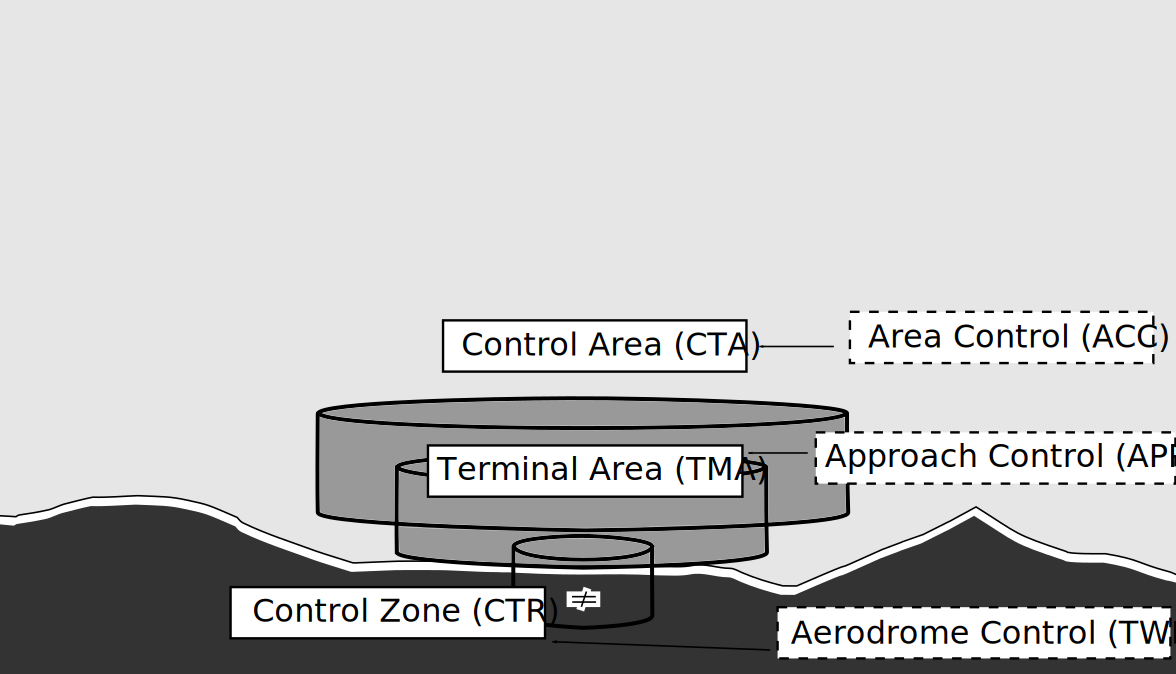
\includegraphics[width=0.8\textwidth]{figures/airspace.png}
    \caption{Airspace - \textcolor{red}{z prezentace 2011 ATM Lesson Plans/ATM 1-1 General Air Traffic Services podle \cite[Chapter 2.5]{annex11} - překreslit!}}
    \label{fig:airspace}
\end{figure}

\begin{figure}[h]
    \centering
    \includegraphics[width=0.8\textwidth]{figures/cta.png}
    \caption{CTA - \textcolor{red}{z prezentace 2011 ATM Lesson Plans/ATM 1-1 General Air Traffic Services podle \cite[Chapter 2.10]{annex11} - překreslit!}}
    \label{fig:cta}
\end{figure}

\begin{figure}[h]
    \centering
    \includegraphics[width=0.8\textwidth]{figures/airspace2.png}
    \caption{Airspace - \textcolor{red}{z prezentace 2011 ATM Lesson Plans/ATM 1-2 General Air Traffic Control Service \cite[Chapter 2.10]{annex11} - překreslit!}}
    \label{fig:airspace2}
\end{figure}

\subsubsection{Area Control Service}
Area Control Service is an ATC service provided by area control centre (ACC) responsible for flights in Control Areas (CTA). Normally ACC is identified by the name of a nearby city, area or landmark. Smaller countries usually have one ACC, but many larger countries are controlled by several of them. ACCs usually control aircrafts in their en-route phase of flight. The ACC may be also responsible for flights to and from smaller aerodromes with no separate approach control service. \cite[Chapter 3.2]{annex11}

\subsubsection{Approach Control Service}
Approach Control Service (APP) is ATC service that is responsible for the part of CTA and CTR required by arriving or departing controlled flights (TMA). The primary functions of APP is sequencing arriving aircrafts and assisting departing aircrafts becoming established on course. The arrival and departure functions can be divided into several positions on busy aerodromes. APP is usually identified by the name of the aerodrome which it is serving, but sometimes it's not colocated with TWR and is at distant ACC location. When no separate ACC exists, approach control service is provided by ACC or TWR. \cite[Chapter 3.2]{annex11}

\subsubsection{Aerodrome Control Service}
Aerodrome control service is provided by a control tower (TWR) and is responsible for aircraft landing and taking off. It's also responsible for VFR flights in the CTR and for preventing collisions between aircrafts on the manoeuvring are of the aerodrome. \cite[Chapter 3.2]{annex11}

\textcolor{red}{POKRAČOVÁNÍ: KAPITOLA 3 Z PREZENTACÍ!!!!!}

\textcolor{red}{z pohledu prostoru/z pohledu kontroly}

\textcolor{red}{v každou chvíli řídí letadlo jeden subjekt a místo a čas předání kontroly je jesně definované - kdy a jak?}

The controlled airspace can furthermore be classified as Class A-G. \cite[\textcolor{red}{kapitola}]{nolan} \textcolor{red}{popis jednotlivých classes podle nolana}

\textcolor{red}{Pro řízení v terminální oblasti nás zajímají všechny druhy řízení/prostoru, Agentfly má zatím jen ACC v CTA?}

\begin{figure}[h]
    \centering
    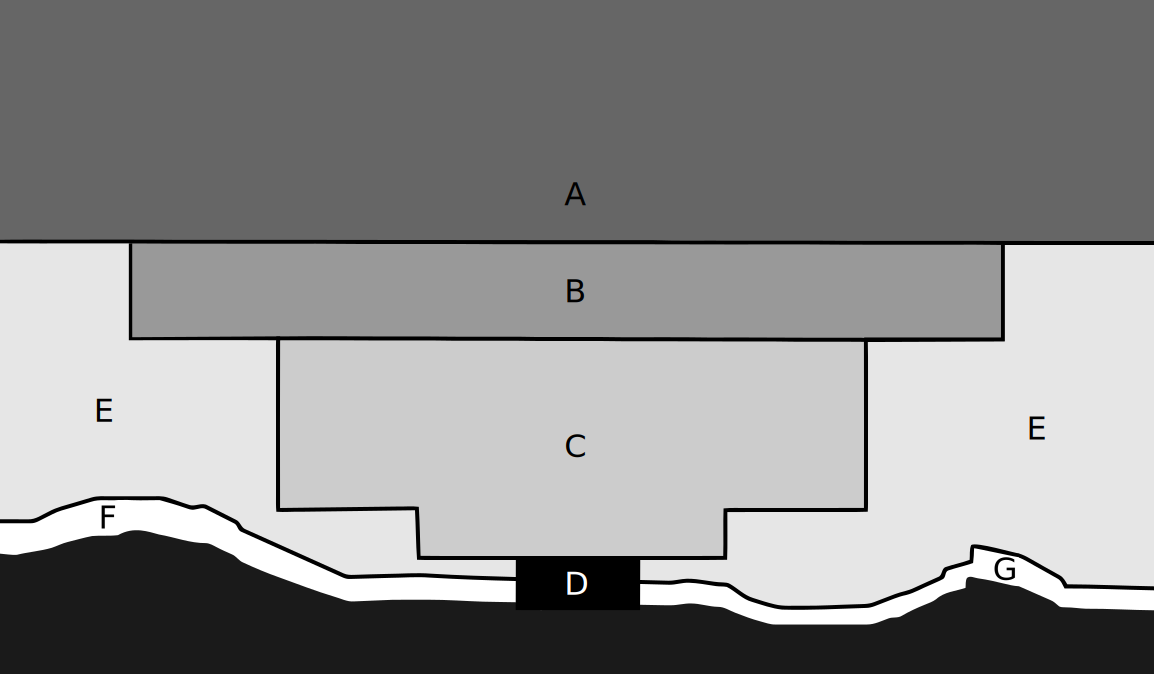
\includegraphics[width=0.8\textwidth]{figures/classes.png}
    \caption{Airspace Classification - \textcolor{red}{z prezentace 2011 ATM Lesson Plans/ATM 1-2 General Air Traffic Control Service \cite {nolan} - překreslit!}}
    \label{fig:classes}
\end{figure}

\textcolor{red}{SID a STAR routy?}
%!TEX root = index.tex
\chapter{Data}
\section{Atlanta Tracon}
\section{Hartsfield–Jackson Atlanta International Airport}
\section{SID + STARs}
\section{Flights}


% v agentfly počítáme pouze s  \item[IFR] Instrument flight rules lety \item[VFR] visual flight rules nás nezajímají

% %\textcolor{red}{v každou chvíli řídí letadlo jeden subjekt a místo a čas předání kontroly je jesně definované - kdy a jak?}


% %\textcolor{red}{Pro řízení v terminální oblasti nás zajímají všechny druhy řízení/prostoru, Agentfly má zatím jen ACC v CTA?}

% do implementace : proč používáme které classes v agentfly

% \subsection{Hartsfield–Jackson Atlanta International Airport}
% Hartsfield–Jackson Atlanta International Airport (ICAO code KATL) has been the world's busiest airport by passenger traffic since 1998 with more than 94 million passengers in 2013. It has also the most landings and take-offs since 2005. The airport has 207 domestic and international gates which is the most at any airport. \cite{atlanta}
%  Proč zvolena pro testy Atlanta...

%!TEX root = index.tex
\chapter{AgentFly}

The AgentFly system is a large-scale high-fidelity distributed multi-agent simulation software. \cite{agentfly-enroute} Its goal is in simulating en-route sector controllers. The simulation combines time-stepped and event-driven simulation approaches. \cite{agentfly-atm} The time-stepped simulation is used for simulating the environment, weather and movement of the planes in space. Default time step used in simulation is set to twelve seconds but can be changed. This allows for faster than real-time simulation. The event-driven approach is used for simulation of the deliberation and communication between pilots and air traffic controllers. These pilots and air traffic controllers are modelled as independent agents.

\section{Air Traffic Model}

The AgentFly's simulation model consists four types of agents: pilot, airplane, visualization and ATC. The airplane agents model the flight itself, it computes it's movement in space using the Base of Aircraft Data (BADA) which is a database of mathematical models that describe the behaviour and performance of modelled aircraft. \cite{bada} The visualization agents show the results of the simulation to the user. The air traffic itself is modelled using pilot and ATC agents.

\subsection{Pilot}

The aircraft in the simulation are operated by pilots who are modelled as pilot agents. Every flight is modelled by a single agent. These agents are event-driven and react to events sent from air traffic controllers. The pilot models the duration of performing the order by waiting for specified amount of time and then replying the ATC confirming the request has been processed and applied.

The pilot agent maintains internal flight plan that contains future intentions and actions of the pilot and therefore describes the precise future flight path of the plane. It consists of waypoints defining the flight route which are connected with elements that describe how the airplane's position, altitude, speed and other characteristics change between the waypoints. When the pilot receives request from ATC, the agent applies the requested change to the flight plan and recomputes new flight states. If there are no instructions from the air traffic controller, the pilot just follows the precomputed flight plan.

The pilot's flight plan uses GPS coordinate system to describe the movement of the plane because it corresponds to the real movement of the plane in 3D space.

\subsection{Controller}
\subsubsection{ATA}
\subsubsection{RSide}

\subsubsection{Workload}

One of AgentFly's main goals is to be able to realistically model the workload of the air traffic controller while he/she performs the tasks needed to keep the traffic separated. This allows to test changes linked to implementing new control procedures in National Airspace System (NAS). Instead of running the simulation with humans (pilots and ATCs) the simulation can be done in AgentFly only, saving both time and expenses.

The ATC's workload is modelled using the Multiple Resource Theory by Christopher D. Wickens, more specifically the workload model developed by McCracken and Aldrich who divide the resources to Visual, Cognitive, Auditory and Psychomotor (VCAP model). \cite{agentfly-enroute} The visual and auditory resources serve for input processing, cognitive resource describes how much internal information processing is required and the psychomotor component describes physical actions as output. The simulated ATC has pools of these resources and each task performed by the ATC requires some of them for specified amount of time (for example typing on keyboard uses psychomotor resource, listening to pilot radio uses auditory resource). No resource can be used by more than one tasks at any time, this means that the controller cannot for example listen to two things at once etc. Using this model the system can measure if the controller is able to process all necessary tasks on time or if the ATC is overloaded.

\subsection{Communication}
%The agents communicate to one another using a sector radio. The sector radio is half duplex - everyone hears everything but only one agent can speak at the same time.



\section{Visualization}
AgentFly system contains modules for advanced 2D and 3D real-time visualization that allows user to monitor and interact with the process of simulation. The visualization is 
implemented using \texttt{OperatorAgent}s. Every one of those agents represents one visualization window and can run on different machines in distributed environment. The information shown in \texttt{OperatorAgent} are shown using layers. Every layer is handled by \texttt{LayerProvider} that creates the representations of objects that will be rendered on the layer.

Two types of windows are usually used in the system, one of them shows 3D model of the Earth and all simulated aircraft flying above the surface at given moment, this serves as a view of real-world situation. Second type of visualization is 2D representation of radar screen of a particular controlled sector. The radar screen shows the sector boundary, aircraft flying in and around the sector and plenty additional information like log of radar communication, graphs of controller workload etc. There are usually multiple radar windows shown for multiple sectors that are being controlled by the simulated ATC.

\section{Used Units}
% The AgentFly system uses two coordinate systems: GPS coordinate system and stereographic
% coordinate system.
% The GPS coordinate system is used to represent positions of aircraft, their flight waypoints
% a fixes. The sectors are also represented in GPS coordinate system. The stereographic 
% coordinate system is created by projection of spherical GPS positions on a plane. Each sector
% in the AgentFly has its own stereographic projection of the world. The stereographic
% coordinate system and the GPS coordinate system have one common point called projection
% point. This projection point could be understood as position of sector radar in AgentFly
% system. The stereographic projection displays sphere on the plane with several compromises.
% E.g., when an aircraft is flying far away from the projection point, it is seemed as
% turning even if flying straight or it is seemed to fly slower than it actually is.
%!TEX root = index.tex

\chapter{Flights Scheduling}

\red{TODO}
% že to je zjednodušení problému na 1 rwy
% co je vlastně kritérium
% různé pořadí různých tříd má různé trvání
% popis obrázků plánů
% posun jen doprava ne dřív
% není to project schedulling protože tady to není jednosměrně, když jsou sloty opačně, tak platí jiná podmínka
% nemůžu použít nic z KOčka - popsat co a proč
% nemůžu použít online algoritmy
% většina z nich počítá s tím, že arrival time a release time jsou stejné, u mně jsou různé,
% Shortest processing time first nemůžu použít, protože processing times nejsou konstantní
% není preempce 
%nejde nám o optimální řešení ale good enough které se podobá reálnému řídícímu

%definice ETA, EETA (earliest), DETA (delayed eta
%uvod ze ted bude vysvetleni jak vypada plan a potom prehled jednotlivych planovacich metod


\section{Runway Plan Visualization}

Runway Plan Visualization module was designed to provide the ATC controller representation of the runway plan that is quick and easy to comprehend. The slots planned for approach are displayed horizontally with a timeline at the bottom with highlighted one and five minute marks.

Above the timeline there are rows representing individual runway plans. Headline of each runway plan is shown on the left side with the number of the runway on the top and names of every weight class in corresponding color shown below. Plans of different runways planned by the same algorithm are divided by gray dashed border. Plans of different runways planned by different algorithms are divided by solid black border.

Each slot in the plan is represented by a vertical green bar with a dark green line in it. The dark green line shows the exact time of expected arrival to the runway and the green bar surrounding it shows the interval of possible arrival as defined by the precision of arrival estimation. Flight ID is shown on the top, the color of the text indicates the weight class of the aircraft. Below the flight ID, gray wake turbulence intervals are shown for every weight class in the same order as in the plan headline. If the wake turbulence interval is active (there is an following airplane scheduled after the current slot), the corresponding interval is colored in the color of following airplane's weight class.

If there is a collision between the slots, active wake turbulence interval of the preceding slot and the slot itself of the following flight are shown in red color. If a slot is delayed, vertical orange line marks the time of original ETA and is connected to the delayed ETA with horizontal orange line. In multi-runway scenarios, earliest ETA among all runways is marked by dotted orange line and is again connected with the delayed ETA with horizontal dotted line. This way the controller can distinguish which part of the delay is caused by the order of slot on the runway and which part of the delay is the runway selection responsible for.

\section{Slot Selection}

\red{TODO}
% pokud vede z aktuální pozice jen jedna star, tak stačí plánovat na jedné rwy:
%zminit, že lze planovat více algoritmy a porovnávat jejich výstup

\subsection{Algorithm 1}

\begin{figure}[h]
    \centering
    \includegraphics[width=\textwidth]{figures/rwy-in-place.png}
    \caption{Example of runway plan with colliding slots}
    \label{fig:rwy-in-place}
\end{figure}

An example of a plan generated by Algorithm 1 is shown in Figure \ref{fig:rwy-in-place}. This algorithm is the simplest of all implemented, it doesn't perform any deliberation on where to put the slot in the plan and simply places it in the time the aircraft is expected to arrive, ignoring possible collisions with other aircraft. This algorithm is obviously no good for actual use and serves only for comparison to other algorithms and to allow analysing of the traffic flow: it shows how many collisions there are or if the planes arrive to the runway periodically or in groups.

\subsection{Algorithm 2}

\begin{figure}[h]
    \centering
    \includegraphics[width=\textwidth]{figures/rwy-end.png}
    \caption{Example of runway with slots in the order of plane's first appearance}
    \label{fig:rwy-end}
\end{figure}

Second algorithm is the simplest one that guarantees no collisions will take place between aircraft. When new plane appears on radar screen it's slot is created after all previously planned slots and not sooner than at the plane's minimal estimated time of arrival.

Figure \ref{fig:rwy-end} shows an example of a plan generated by this algorithm. It is clearly visible that unnecessary delays can occur when the interval between when the plane shows on the radar and its ETA differ from plane to plane. This can happen when the arrival routes have different lengths. Approach route for airplane heading directly to runway will be much shorter than for airplane arriving from opposite direction, because such plane must first fly around the airport before landing. \red{ref to figure with KATL approach routes} In the example shown on Figure \ref{fig:rwy-end} flight \texttt{TRS753} will arrive more than 5 minutes late because it appeared on the radar screen later than flights \texttt{TRS1341} and \texttt{DAL1946}.

\subsection{Algorithm 3}

\begin{figure}[h]
    \centering
    \includegraphics[width=\textwidth]{figures/rwy-fill-voids.png}
    \caption{Example of runway plan with slots fixed in place}
    \label{fig:rwy-fill-voids}
\end{figure}

Algorithm 3 creates the slot for arriving airplane in the first empty space following planes estimated arrival time the slot fits in. The wake turbulence separation minima is taken into account for both preceding and following slot so no collisions between slots occur. The advantage of this this algorithm is its simplicity and the fact that the planed slots are fixed. This means that if the controller assigns a slot to airplane and clears it for approach he/she doesn't have to alter the airplane's clearance and can focus on other arriving aircraft.

An example of a plan generated by Algorithm 3 is shown in Figure \ref{fig:rwy-fill-voids}. In comparison to plan generated by previous algorithm (\ref{fig:rwy-end}) it is apparent that flights \texttt{TRS753}, \texttt{DAL1304} and \texttt{DAL1799} can land sooner than \texttt{TRS1341} even though they entered the controlled area later.

\subsection{Algorithm 4}

\begin{figure}[h]
    \centering
    \includegraphics[width=\textwidth]{figures/rwy-eta-order.png}
    \caption{Example of runway plan that preserves the order of estimated time of arrival}
    \label{fig:rwy-eta-order}
\end{figure}

Fourth algorithm was implemented in two variants, the first one schedules the slots in a way that strictly preserves the order of estimated time of arrival. If the slot doesn't fit, any already planned slots following this one are delayed. If there is a continuous string of planes scheduled for approach one after other and new, early arriving plane appears on the radar screen the controller using this algorithm will squeeze the plane in and postpone the planes following in the string. This prevents a situation where the new airplane would wait for all the planes in the string to land first and potentially deplete its fuel supply. On the other hand the controller may need to postpone a significant number of previously planned aircraft which would take a considerable amount of time.

The second variant is not strict with the order according to ETA. It finds the place where the new slot would fit by the ETA, but inserts it only if the delay of the following slot after the new slot is inserted is smaller than the delay of the new slot would be if it was placed after the following slot. Otherwise it tries to insert the new slot after the slot following it and so forth until the condition is met. This serves as a local optimization of the maximal delay and helps the algorithm to cope with flights with alternating weight classes.

The example plans generated by this algorithm are shown in Figure \ref{fig:rwy-eta-order}, first row contains result of first variant, second row contains second variant. First \texttt{01M} was inserted, followed by \texttt{03J}. Then \texttt{02J} arrived with earlier ETA than \texttt{01M}. First variant places the \texttt{02J} to the beginning of the plan and significantly shifts \texttt{01M} and \texttt{03J}. Second variant compares the delay of \texttt{01M} behind \texttt{02J} with delay of \texttt{02J} behind \texttt{01M}. The second delay is smaller and therefore the algorithm doesn't place \texttt{02J} before \texttt{01M}, but continues after \texttt{01M}, here it performs the same comparison between \texttt{02J} and \texttt{03J} and this time placing \texttt{02J} before \texttt{03J}. The algorithm keeps inserting additional slots using this local optimization finally producing much shorter plan than first variant of the algorithm would.

\subsection{Algorithm 5}

\begin{figure}[h]
    \centering
    \includegraphics[width=\textwidth]{figures/rwy-bab.png}
    \caption{Comparison between Algorithm 4v1 (first row) and three variants of Algorithm 5}
    \label{fig:rwy-bab}
\end{figure}

Algorithm 5 is an algorithm commonly used in combinatorial optimization and is called Branch and bound. \cite{bab} The algorithm is used here in three different variants, each optimizing different criterion. First variant minimizing $C_{max}$, the schedule length also called makespan, which is equal to completion time of last task.  Second variant minimizes $W_{max} = max\{w_j\}$, maximal waiting time. The waiting time is defined as the difference between release time and start time of the task, in this instance difference between required time of arrival and actual time of arrival. Third variant minimizes $\sum{w_j}$, the sum of all waiting times.

Figure \ref{fig:rwy-bab} shows a comparison between first variant of Algorithm 4 and the three variants of Algorithm 5. The first variant is in the second row, second variant is in the third row and the third variant is in the last row. Note that all three versions perform significantly better than Algorithm 4v1. The difference between the tree variants is small with variant 1 and 3 even producing the exact same plan in this instance.

\begin{figure}[h]
    \centering
    \includegraphics[width=0.7\textwidth]{figures/rwy-proof.png}
    \caption{Example of adding later slot causing changes in plan before its ETA}
    \label{fig:rwy-proof}
\end{figure}

Unfortunately there are two serious problems with Algorithm 5 that prevent its use in real world application.

The first one is that it doesn't keep the relative order of previously planned slots. This is caused by the fact that the algorithm is an offline algorithm and recomputes the whole plan from scratch every time new slot needs to be added. This is illustrated in Figure \ref{fig:rwy-proof} where addition of slot for flight \texttt{05M} caused the order of slots for \texttt{01M}, \texttt{02J} and \texttt{03J} to change. Changing the order of flights scheduled on a route to one runway would result in need of special behaviour that would allow the plane to leave the route, wait in a separate area until the following aircraft flies past on the route and then return back to the route. And because the complete replanning takes place every time new plane appears on a screen it could happen that two flights would switch their place in the sequence back and fort multiple times before reaching runway.

Additionally the planed delay may decrease for any given plane in time (see \texttt{02J} in Figure~\ref{fig:rwy-proof}). But if the plane already performed certain manoeuvre to slow it down to accommodate the delay prescribed by the previous plan, it may be impossible to speed up to reach the runway in time planned by the updated plan, even so it would be able to do so before the hold-up.

\begin{table}[h]
  \centering
\begin{tabular}{ | l || r | r | r | r | r | r | }
\hline
			& 10 slots	& 11 slots	& 12 slots	& 13 slots	& 14 slots	\\
\hline
Version 1	& $< 1s$	& $3s$		& $37s$		& –			& –			\\
Version 2	& $< 1s$	& $< 1s$	& $< 1s$	& $7s$		& $33s$		\\
Version 3	& $< 1s$	& $4s$		& $45s$		& –			& –			\\
\hline
\end{tabular}
  \caption{Run times of the three variants of Branch and bound algorithm}
  \label{tab:alg5-runtime}
\end{table}

The second disadvantage of this algorithm is also linked to the need to recompute the whole plan with each slot addition and it is the computational complexity of the Branch and bound algorithm.

The algorithm enumerates possible solutions in a systematic way that ensures the optimum will be found eventually. To prevent searching through the whole state space, upper and lower bounds are used to prune the unpromising branches from the search tree. The minimal solution found so far can act as an upper bound pruning all branches with partial plans whose criterion value is already bigger or equal to the optimum. This is especially beneficial for the second variant minimizing maximal delay among all slots, because the pruning takes place early on in the search tree, eliminating many non-optimal solutions.

For optimizing makespan any empty voids in the plans can be used as a bound for the solution. This can be done if the slots are ordered according to their ETA. In such case if the ETA of the next added slot is later than the end of the previous slot and forms an empty void before it, the optimal solution lies in a tree rooted by the added slot. This is because rearranging the order of previous slots wouldn't allow the next slot to start sooner than it starts in the current partial solution. This bound cannot be used in variants 2 and 3, because rearranging previously planned slots can still improve maximal and total delay.

The sum of tasks that remain to be planned added to the length to the current partial plan can serve as an upper bound to the solution. If this value exceeds the value of the minimal solution found so far it is obvious that planning the remaining tasks cannot result into better result and current sub-tree can be pruned. This bound cannot be effectively used in this planning problem, because the size of the slots isn't constant and therefore the size of the sum depends on the order in which the slots are added to the plan. And finding the order of the slots that produces the smallest sum equals to the planning problem itself.

The previously mentioned restrictions limit the benefits of pruning and the algorithm must therefore search through a significant part of the state space which makes it slow. The Table \ref{tab:alg5-runtime} shows the runtime for rather small instances of the planning problem and shows that the algorithm can't be successfully used for faster than real time simulation.

\section{Runway Selection}

When the configuration of STARs and the airport allows the planes to land on one of several runways, the air traffic controller must not only decide on the order in which the airplanes land on the runway but also on which plane lands on which runway.

The procedure for runway selection goes as follows: For every runway the arriving plane can land on, new plan is created incorporating the slot for the incoming aircraft. The plans are created using the single-runway algorithms introduced in previous section. Than all the created plans are compared using one of the criteria presented below, the optimal plan is used for the corresponding runway and other plans are thrown away and the runways keep their previous plans not containing the slot of the newly arriving plane.

First criterion used to compare runway plans is ETA of the new slot. The air traffic controller obviously wants the airplanes to land as soon as possible and this criterion is fucused on just that. It compares the arrival times of the newly added slot and directs the airplane to the runway with lowest time. This way the airplane may fly to a runway which is further away if the runway is less utilized and allows for earlier landing than a runway that has the shortest route.

Second criterion guides the airplane to the runway with the smallest makespan after the slot addition. This way the controller keeps all runways equally occupied because new airplane is always routed to the least occupied runway (that is to the one with smallest makespan).

Third and fourth criteria for runway selection are total respectively maximal delay of all slots planned on the runway. The rationale for using these criteria is the same as for planning on single runway mentioned above.

\section{STAR Selection}

Apart from the situation where there are multiple STARs leading to multiple runways, there are also cases where there are multiple routes leading to the same runway leading to the same runway and the air traffic controller must decide which route to use. For example see Figure \red{routy okolo KATL} where airplane arriving from northeast through fix \texttt{FLCON} can land on runway \texttt{9R} flying along either route north of the airport or south of the airport.

The decision is made as follows: when there are multiple routes to one runway arriving flight can take, the one with shortest estimated duration is used for planning. Then schedulling on multiple runways is performed the same way as was described above. If the runway with multiple routes leading to it is selected deliberation on which of the routes to take is carried out. If the slot assigned to the arriving flight has a delay from the ETA of the shortest STAR (because the runway is busy with other flights at the moment) and the delayed ETA is bigger than that of another route with longer duration, this route is used instead of the shortest.

This basically means that if the runway is free, the plane takes the shortest route, but if the flight needs to be delayed, the controller preffers that the plane takes a longer route to take away from the delay rather than hold in one place and taking the short route. The plane needs to be delayed anyway and this way it at least doesn't occupy the holding pattern and instead flies along a different route.
%!TEX root = index.tex
\chapter{Implementation}

\label{section:implementation}
%Then the air traffic controller module is implemented. The module provides the means for controlling aircraft in the approach phase of the flight. The controller schedules the incoming flights to available runways in an effort to land them quickly and safely. Several different scheduling algorithms are implemented each offering different approach for arranging the flights for landing. Also the current methods of simulating aircraft in the AgentFly system need to be extended to allow for simulation of the approach phase of the flight including two methods of delaying the flights before they can commence the final approach to runway. The first one is holding pattern that is used when the flight needs to be delayed by a greater amount of time. The second if horizontal diversion manoeuvre which delays the aircraft by a lesser amount of time by diverting the plane from its flight plan and therefore prolonging its route.
% cilem implementovat moduly ktere naplanuji prijezd aby se nepotkaly na letisti! a aplikovat tak aby tak letadla fakt letela
\red{TODO}

\section{Data Processing and Visualization}

\red{TODO}

\subsection{Runway Plan Visualization}

The visualization of runway plans is implemented in \texttt{RunwayPlanVisualModule} and its inner class \texttt{GraphicRunwayPlan}. \texttt{VisualModule}s are used in AgentFly to display additional information on controllers radar screen. When the runway plans are updated by the simulated ATC controller, \texttt{RunwayPlanVisualModule} converts the updated plans to their graphical representation described by instances of \texttt{GraphicRunwayPlan} and draws them on the radar screen.

The implementation of visualization is general and can display plans for any number of runways created by any number of planning algorithms. There is a scrollbar at the bottom of the visualization window that allows plans that are longer than viewport to be shown. The visual output is described in \ref{section:runway-visualization}.

\subsection{Approach Routes}

Approach routes (STARs) are provided in proprietary formatted CSV file. The routes are defined by short segments and links connecting those segments. \texttt{ApproachRoutes\-Csv\-ScenarioPlayer} reads the route definitions, creates their representation and publishes them using \texttt{SharedObjectHolder} so that they can be used through the whole simulation.

The routes are stored in a data structure \texttt{ApproachRoutesData} that allows the routes to be found according to their star fix or the runway they're leading to. The routes themselves are represented by \texttt{ApproachRoute}. Each route contains information about runway it leads to, individual waypoints on the route, defined holding patterns along the route and estimated route duration and accuracy interval of the estimation. Waypoints are represented by \texttt{ApproachRouteWaypoint} defining the waypoint's name, position and altitude and speed interval passing planes must fit in.

Rendering of the approach routes in real-world 3D visualization is provided by \texttt{Approach\-Routes\-LayerProvider}. It can show either only the routes, or routes with waypoint names or complete route information with the altitude and speed intervals. The output of the visualization is shown in Figure \ref{fig:routes}.

\subsection{Wake Turbulence Separation Intervals}

Wake turbulence separation intervals are provided in a text file. This data file is processed by \texttt{WakeTurbulenceDataScenarioPlayer} and shared with the simulation environment through \texttt{SharedObjectHolder}. The data are stored in \texttt{WakeTurbulenceData} which provides methods that return the separation given the wight classes of the preceding and following airplanes.

\subsection{Airplane Trails}

\texttt{AirplaneTrailLayerProvider} serves as additional visual aid that allows the user to easily analyze the course of the aircraft's flight. It subscribes to aircrafts' position updates and gradually draws a line through all of them. After the plane lands entire trail of the flight is shown in the real-world simulation window. The number of trails shown on screen after their airplanes landed can be set through configuration file.

\section{Scheduling}

The TMA air traffic controller's behavior is implemented in module \texttt{EomAtaStarApplication}. The module keeps an internal plan of which plane is scheduled to land on which runway at which time. When a new plane appears on the sector radar screen, the landing is scheduled and the pilot is commanded to use selected STAR for approach. Then the controller monitors the progress of the flight and either updates the plan to correspond with the reality or orders the pilot to perform such manoeuvres to arrive to the runway at prescribed time. The following section describes the process of approach scheduling. See the corresponding flowchart in Figure \ref{fig:flowchart1}.

When a new plane appears on screen \texttt{EomAtaStarApplication} must select to which runway through which STAR the plane should be heading and create a new slot in the runway plan. First, all routes that the plane can take to the airport are filtered.

\subsection{STAR Selection}

There are several possible scenarios for the scheduling and STAR selection. If only single STAR is available, the situation is simple. Controller schedules the airplane to land on the runway the STAR leads to using one of the algorithms described in \ref{section:slot-selection} and orders the pilot to use the STAR for approach.

If there are several STARS leading to different runways, controller must select one first. This is done using one of the multi-runway scheduling algorithms described in \ref{section:runway-selection}.

\pgfdeclarelayer{marx}
\pgfsetlayers{main,marx}

\providecommand{\cmark}[2][]{\relax}
\providecommand{\cmark}[2][]{
  \begin{pgfonlayer}{marx}
    \node [nmark] at (c#2#1) {#2};
  \end{pgfonlayer}{marx}
  } 

\begin{figure}[H]
    \centering
\begin{tikzpicture}[
    >=triangle 60,
    start chain=going below,
    node distance=6mm and 53mm,
    every join/.style={norm},
    ]

\tikzset{
  base/.style={draw, on chain, on grid, align=center, minimum height=4ex},
  proc/.style={base, rectangle, text width=9em},
  test/.style={base, diamond, aspect=2, text width=5em},
  term/.style={proc, rounded corners},
  coord/.style={coordinate, on chain, on grid, node distance=6mm and 25mm},
  nmark/.style={draw, cyan, circle, font={\sffamily\bfseries}},
  norm/.style={->, draw, black},
  it/.style={font={\small\itshape}}
}
\node [term, fill=green!20]	(t1)	{New airplane on screen};
\node [proc, join]			{Filter applicable STARs};
\node [proc, join]			{Schedule slot to all available runways};
\node [proc, join]			{Find best runway and STAR combination};
\node [term, join, fill=orange!25]{\ding{183} Apply selected STAR};
\node [term, join, fill=orange!25]{\ding{182} Delay all updated slots};

\node [term, fill=black!20]	{\ding{182} Delay all updated slots};
\node [test, join]	(x4)	{Any slots left?};
\node [term, fill=orange!25](t7){\ding{184} Match airplane sgPlan to arrival slot};
\node [term, fill=orange!25](t8){\ding{108} Update runway plan visualization};

\node [term, fill=green!20, right=of t1](t2){Airplane wants to entry TMA sector};
\node [term, join, fill=orange!25]{\ding{184} Match airplane sgPlan to arrival slot};
\node [test, join]	(x1)	{Applied any delay manoeuvre?};
\node [test]		(x2)	{Applied diversion manoeuvre?};
\node [test]		(x3)	{Applied holding in sector?};
\node [proc]		(t3)	{Reject entry, apply holding first};

\node [proc, right=of x1](t4){Approve entry};
\node [proc, right=of x2](t5){Approve entry, apply diversion in TMA};
\node [proc, right=of x3](t6){Approve entry, apply holding in TMA};

\node [term, right=of t3, fill=orange!25](t9){\ding{182} Delay all updated slots};

\node [term, fill=green!20, right=of t2]	{Airplane landed};
\node [proc, join]			{Remove slot from runway plan};
\node [term, join, fill=orange!25]{\ding{108} Update runway plan visualization};

\node [coord, right=of x1]	(c1) {}; \cmark{1}
\node [coord, right=of x2]	(c2) {}; \cmark{2}
\node [coord, right=of x3]	(c3) {}; \cmark{3}
\node [coord, left=of x4]	(c4) {}; \cmark{4}
\node [coord, right=of t5]	(c5) {}; \cmark{5}
\node [coord, left=of t8]	(c6) {}; \cmark{6}
\node [coord, right=of x4]	(c7) {}; \cmark{7}
\node [coord, right=of t4]	(c8) {}; \cmark{8}
\node [coord, right=of t6]	(c9) {}; \cmark{9}

\node [coord, right=of t9]	(cb) {}; \cmark{b}

\path (x4.south) to node [near start, xshift=1em] {yes} (t7);
	\draw [*->,black] (x4.south) -- (t7);

\path (x1.south) to node [near start, xshift=1em] {yes} (x2);
	\draw [*->,black] (x1.south) -- (x2);
\path (x2.south) to node [near start, xshift=1em] {no} (x3);
	\draw [o->,black] (x2.south) -- (x3);
\path (x3.south) to node [near start, xshift=2.2em] {en-route} (t3);
	\draw [*->,black] (x3.south) -- (t3);

\path (x1.east) to node [near start, yshift=1em] {no} (c1); 
	\draw [o->,black] (x1.east) -- (t4);
\path (x2.east) to node [near start, yshift=1em] {yes} (c2); 
	\draw [*->,black] (x2.east) -- (t5);
\path (x3.east) to node [near start, yshift=1em] {TMA} (c3); 
	\draw [*->,black] (x3.east) -- (t6);


\path (x4.west) to node [near start, yshift=1em] {no} (c4); 
	\draw [o->,black] (x4.west) -- (c4) -- (c6) -- (t8);
\draw [->,black] (t7.east) -| (c7) -- (x4);
\draw [->,black] (t6.east) -- (c9) -- (cb) -- (t9);
\draw [->,black] (t3.east) -- (t9);
\draw [->,black] (t4.east) -- (c8) -- (c5);
\draw [->,black] (t5.east) -- (c5) -- (c9);

\end{tikzpicture}
    \caption{Flowchart showing simplified processes of ATC in TMA sector as implemented by \texttt{EomAtaStarApplication}.}
    Algorithm entry points responding to events from the simulation framework are shown in green. Internal subroutines' entry points are shown in gray and the subroutine calls are orange. The flowchart continues in Figure \ref{fig:flowchart2}. The subroutine numbers don't represent order, they are only visual aid to match routine definition and call.
    \label{fig:flowchart1}
\end{figure}


\begin{figure}[h]
    \centering
\makebox[\textwidth][c]{
\begin{tikzpicture}[
    >=triangle 60,
    start chain=going below,
    node distance=6mm and 53mm,
    every join/.style={norm},
    ]

\tikzset{
  base/.style={draw, on chain, on grid, align=center, minimum height=4ex},
  proc/.style={base, rectangle, text width=9em},
  test/.style={base, diamond, aspect=2, text width=5em},
  term/.style={proc, rounded corners},
  coord/.style={coordinate, on chain, on grid, node distance=6mm and 25mm},
  nmark/.style={draw, cyan, circle, font={\sffamily\bfseries}},
  norm/.style={->, draw, black},
  it/.style={font={\small\itshape}}
}

\node [term, fill=black!20]	(t0)	{\ding{183} Apply selected STAR};
\node [test, join]			(x4)	{Sector the plane is in?};
\node [proc]				(t2)	{Order pilot to apply STAR through radio};
\node [proc]				(t3)	{Contact enroute ATC through landline};

\node [term, fill=black!20, right=of t0]{\ding{184} Match airplane sgPlan to arrival slot};
\node [test, join]			(x1)	{Plane enter(ed/ing) sector?};
\node [test]				(x2)	{Update slot/delay flight?};
\node [test]				(x3)	{Delay size};
\node [proc]				(t1)	{Apply holding pattern};

\node [proc, right=of x1]	(u1)	{Wait for plane entry};
\node [proc, right=of x2]	(u2)	{Update slot in runway plan};
\node [proc, right=of x3]	(u3)	{Apply diversion manoeuvre};

\node [coord, right=of x1]	(c1)	{}; \cmark{1}
\node [coord, right=of x2]	(c2)	{}; \cmark{2}
\node [coord, right=of x3]	(c3)	{}; \cmark{3}
\node [coord, left=of x4]	(c4)	{}; \cmark{4}
\node [coord, left=of t3]	(c5)	{}; \cmark{5}

\path (x1.south) to node [near start, xshift=1em] {yes} (x2);
	\draw [*->,black] (x1.south) -- (x2);
\path (x1.east) to node [near start, yshift=1em] {no} (c1); 
	\draw [o->,black] (x1.east) -- (u1);

\path (x2.south) to node [near start, xshift=2.8em] {delay flight} (x3);
	\draw [*->,black] (x2.south) -- (x3);
\path (x2.east) to node [near start, yshift=1em, xshift=0.5em] {update} (c2); 
	\draw [*->,black] (x2.east) -- (u2);

\path (x3.south) to node [near start, xshift=2.3em] {$d > 3$min} (t1);
	\draw [*->,black] (x3.south) -- (t1);
\path (x3.east) to node [near start, yshift=1em, xshift=0.6em] {$d \leq 3$min} (c3); 
	\draw [*->,black] (x3.east) -- (u3);

\path (x4.south) to node [near start, xshift=1.5em] {TMA} (t2);
	\draw [*->,black] (x4.south) -- (t2);
\path (x4.west) to node [near start, yshift=1em, xshift=-0.6em] {en-route} (c4); 
	\draw [*->,black] (x4.west) -- (c4) -- (c5) -- (t3);

\end{tikzpicture}}
    \caption{Continuation of the flowchart showing simplified processes of ATC in TMA sector from Figure \ref{fig:flowchart1}.}
    Internal subroutines' entry points are shown in gray.
    \label{fig:flowchart2}
\end{figure}

There are also cases where multiple routes lead to the same runway and the air traffic controller must decide which route to use. For example see Figure \ref{fig:routes}: airplane arriving from northeast through fix \texttt{FLCON} can land on runway \texttt{9R} flying along either route north of the airport or south of the airport.

The decision is made as follows: when there are multiple routes to one runway arriving flight can take, the one with shortest estimated duration is used for planning. Then scheduling on multiple runways is performed as was described in \ref{section:runway-selection}. If the runway with multiple routes leading to it is selected to be used, deliberation on which of the routes to take is carried out. If the slot assigned to the arriving flight has a delay from the ETA of the shortest STAR (because the runway is busy with other flights at the moment) and the delayed ETA is bigger than that of another route with longer duration, this route is used instead of the shortest.

This basically means that if the runway is free, the plane takes the shortest route, but if the flight needs to be delayed, the controller prefers that the plane takes a longer route to accommodate the delay rather than hold in one place and taking the short route. The plane needs to be delayed anyway and this way it at least doesn't occupy the holding pattern and instead flies along a different route.

The plan of approaches of each runway is represented by an instance of \texttt{RunwayPlan}. It contains all scheduled slots on the runway and provides methods for new slot allocation based on the algorithms described in \ref{section:slot-selection} as well as methods that provide information for comparison of the plans for multi-runway scheduling. These return plan makespan, maximal delay among the planned slots, total delay of all planned slots etc. Slots are instances of \texttt{RunwaySlot} and hold flight ID, plane weight class, earliest ETA, target ETA, latest ETA and slot delay.

%\FloatBarrier 

\section{STAR Application}

When the approach is planned, the controller must advise the pilot which route he/she has to use for landing. First the controller determines in which sector the airplane is currently located (see Figure \ref{fig:flowchart2}). Typically this is one of the neighboring en-route sectors, but the airplane might also already be in the TMA sector. If the airplane is in en-route sector, the TMA controller sends event to en-route controller to contact the pilot through radio. If the plane is in the TMA sector, the controller contacts the pilot directly.

The radio communication is provided by \texttt{EomRSideStarApplication} module. The module arranges for the whole process including for the communication itself, delay of the communication, repeated transmissions if the previous tries failed and displaying the message in radio communication window on the radar screen. The message transmitted through radio is represented by \texttt{StarApplicationData}.

\subsection{Flight Plan Update}

On the pilot's side, the radio message is received by module \texttt{EomPilotStarApplication} which applies the STAR to its current flight plan that is represented by \texttt{GpsFlightPlan\-WrapperPolyline}. The flight plan wrapper was extended so it can apply the whole STAR with single replanning. First a common waypoint of current flight plan route and applied STAR is found and the STAR is appended to the flight plan after the common waypoint replacing the original route. Then a list of clearances is created, with required altitudes and speeds at fixes along the STAR. Finally, flight plan is replanned  through the added STAR with restrictions defined by the clearances using BADA model of the plane's behavior.

When the STAR is applied, \texttt{EomAtaStarApplication} gathers all slots that have been updated during the scheduling, including the newly added slot, and ensures that each slot matches the estimated arrival according to the current airplane sgPlan. The process is shown in Figure \ref{fig:flowchart1}. The sgPlan represents the airplane not from the pilots view, but from the controllers perspective. While doing so, more slots can be updated and the process continues until all slots and sgPlans match. When the matching is done, visualization of runway plans is updated.

\section{Sector Entry Check}

Sector entry check is a process that takes place before the hand-off of an airplane to new sector is performed. At this time the plane's sgPlan is available for the first time. For TMA sector the entry check procedure is shown in figure \ref{fig:flowchart1} and works as follows:

Since the sgPlan of plane in entry check is now known, the controller can match the sgPlan and planned slot. While doing so, more slots can be updated and the process continues until all slots and sgPlans match. When the matching is done, the result of matching of the entering airplane is examined. If no delay manoeuvre was performed and only the slot was updated, the entry is approved and hand-off will take place. If horizontal diversion manoeuvre was applied, the entry is approved and TMA controller waits till the plane crosses to TMA sector to perform the vectoring. If holding was applied before the plane crosses border to TMA sector, the entry is rejected and another entry check will take place once the airplane completes its holding in en-route sector and will be about to cross to TMA once again. If the holding pattern was applied after the plane crosses the border of TMA sector, entry is approved and airplane holds inside TMA.

\section{Flow Control}

The duty of the flow control is to make sure, that the airplanes will reach the runway during its assigned time slot. To do that, \texttt{EomAtaStarApplication} must either update the slot to match the sgPlan or delay the plane so the sgPlan will match the slot. The process is shown in Figure \ref{fig:flowchart2}.

First, the controller checks whether the entry check took place and sgPlan is already available and if not, airplane wait for its entry.

If the sgPlan is available, sgPlan arrival interval is determined and compared with the runway plan slot. If the sgPlan interval is smaller than the slot and fits inside it, the slot is shrunk not to occupy unnecessary time on the runway.

If the sgPlan arrival interval is smaller than the runway slot and ends later (the estimated arrival was too optimistic), the slot is shifted later in time and shrunk to fit the arrival interval. This can lead to shifting of slots planned after the current one and these slots will have to be matched to their sgPlans after the matching of current slot is finished. The following slots can be only shifted further in time, the order of the slots is preserved.

If the sgPlan arrival interval is bigger than runway slot and the slot ends sooner than the arrival interval, the slot is enlarged and shifted so it fits the arrival interval. Again, this may lead to the need to shift following slots in the runway plan.

Finally if the sgPlan arrival interval starts sooner than the runway slot (the estimated arrival was pessimistic) no matter if the interval is bigger and smaller than the slot, the controller first tries to shift the slot back in time so it starts at the same time as the arrival interval. This is possible only if there is empty space in the runway plan before the slot. If there is no empty space or the slot can't be moved backwards all the way, the plane must be delayed so the sgPlan arrival interval would fit in the slot. Once the plane is delayed, the runway slot is shrunk or enlarged to fit the updated sgPlan arrival interval.

If the plane needs to be delayed by more than three minutes, holding pattern is used, if the delay is smaller or equal than three minutes, horizontal diversion manoeuvre is used. The tree minute threshold is arbitrary and based on experience, and can be changed to different value. 

\subsection{Vectoring}

Horizontal diversion manoeuvre is performed by \texttt{EomAtaVectoring} module using airplane vectoring. Unlike STAR or holding application, in which the controller tells the pilot what manoeuvre to use immediately ({\em``Hold 5 minutes at fix SINCA''} ) and the pilot incorporates them into his/hers flight plan and performs them at the right time and place, vectoring is performed by the pilot at the exact time he/she received the order through radio ({\em``Turn to heading 270 immediately''} ).

\begin{figure}[h]
    \centering
    
\includegraphics[width=\textwidth]{figures/diversion.png}
    \caption{\red{popis a reference do textu}}
    \label{fig:diversion-implementation}
\end{figure}

This means that the \texttt{EomAtaVectoring} module only computes the geometry of the manoeuvre (when and how much the plane must divert from its flight plan to achieve required delay) and applies it to the sgPlan. The vectoring itself (radio communication with the pilot) takes place later at the time the plane must divert. This is already implemented in AgentFly and used for example in collision avoidance.

\subsection{Holding Pattern}

If the holding pattern needs to be applied to delay the plane's arrival, the \texttt{EomAtaStar\-Application} first needs to decide which holding pattern to use. If there are any published holding patterns on the remaining part of STAR ahead of the plane, the one defined for earliest fix will be used to delay the airplane early on and not at the latest possible moment just before landing.

\begin{figure}[h]
    \centering
    \includegraphics[width=\textwidth]{figures/hold.png}
    \caption{\red{popis a reference do textu}}
    \label{fig:holding-implementation}
\end{figure}

If there is no published holding pattern, the controller creates one ad hoc. He/she tries to create it as early as possible. If the holding pattern would cross the sector border and the plane would therefore cross it back and forth multiple times, the controller first tries to decrease the holding pattern size (and make the plane fly through it more times) and if that doesn't help, he/she then creates the holding further down the route inside the TMA sector.

The application of the manoeuvre itself is done by \texttt{EomAtaHoldingApplication} module. It calculates how much time the plane needs to spend in the holding pattern to achieve desired arrival time at the runway and incorporates the holding pattern into sgPlan.

The communication with the pilot is ensured by \texttt{EomRSideHoldingApplication} and in much the same way as in STAR application, the whole process of the communication is arranged including delay of the communication, repeated transmissions if the previous tries failed and displaying the message in radio communication window on the radar screen. The message transmitted through radio is represented by \texttt{HoldingPatternData} and includes the holding fix information, holding altitude, pattern heading, holding direction, speed and time, when the holding is completed and plane should continue with the approach.

On the pilot's side, the radio message is received by \texttt{EomPilotHoldingPattern\-Appli\-cation} module that applies the holding to its current flight plan, represented by \texttt{GpsFlight\-Plan\-WrapperPolyline}. New waypoints defining the shape of the the holding pattern are added as well as clearances ensuring the holding will be carried out at the right altitude and speed. Finally, flight plan is replanned using BADA model of the plane's behavior.

\section{Airplane Landing}

The last task performed by \texttt{EomAtaStar\-Application} module is checking if the airplane landed at the correct time (shown in Figure \ref{fig:flowchart1}). When event marking that an airplane landed, the controller checks if the touchdown time fits inside. If it doesn't, there has been probably some error during one of the manouvres performed by the pilot before arrival. The airplane arriving outside its slot is logged to be further investigated.

When the check is completed, the controller removes the slot from the corresponding runway plan to minimize the plan's size leading to faster allocation of future slots. Also the runway plans visualization is updated.

%\subsection{Miles In Trails}
%!TEX root = index.tex
\chapter{Testing}
\section{Comparison To Real Air Traffic}
\section{Flight Duration}
\section{Fuel Consumption}
\section{Controller Workload}
\section{Airport/Runway capacity}
%!TEX root = index.tex
\chapter{Conclusion}
\section{Future work}


%!TEX root = index.tex

%\bibliographystyle{abbrv}
%\bibliographystyle{plain}
%\bibliographystyle{psc}
%{
%JZ: 11.12.2008 Kdo chce mit v techto ukazkovych odkazech take odkaz na CSTeX:
%\def\CS{$\cal C\kern-0.1667em\lower.5ex\hbox{$\cal S$}\kern-0.075em $}
%\bibliography{bibliografie}
%}

%!TEX root = index.tex

\cleardoublepage 
\begin{thebibliography}{1}

\bibitem{growth}
ICAO.
\newblock {\em Strong Passenger Results and a Rebound for Freight Traffic in 2014.}
\newblock International Civil Aviation Organization, Montréal, 18 December 2014.
\newblock Available at: \url{http://www.icao.int/Newsroom/NewsDoc2014/COM.48.14.EN.pdf}

\bibitem{atm}
Eurocontrol.
\newblock {\em What is air traffic management} [online].
\newblock European Organisation for the Safety of Air Navigation [cited 2014-11-16].
\newblock Available at: \url{http://www.eurocontrol.int/articles/what-air-traffic-management}

\bibitem{nolan}
M.~S. Nolan.
\newblock {\em Fundamentals of air traffic control}.
\newblock Thomson--Brooks/Cole, Belmont, CA, 4th edition, 2004.

\bibitem{aim}
United States Department of Transportation, Federal Aviation Administration.
\newblock {\em Aeronautical Information Manual - Official Guide to Basic Flight Information and ATC Procedures}.
\newblock United States Department of Transportation, Federal Aviation Administration, 2014.
\newblock Available at: \url{https://www.faa.gov/air_traffic/publications/ATpubs/AIM/}.

\bibitem{doc4444}
ICAO.
\newblock {\em Doc 4444 – Air traffic management}.
\newblock International Civil Aviation Organization, Montréal, 15th edition, 2007.

\bibitem{doc8168}
ICAO.
\newblock {\em Doc 8168 – Aircraft Operations Volume I, Flight Procedures}.
\newblock International Civil Aviation Organization, Montréal, 5th edition, 2006.

\bibitem{annex11}
ICAO.
\newblock {\em Annex 11 to the Convention on International Civil Aviation: Air Traffic Services}.
\newblock International Civil Aviation Organization, 2001.

\bibitem{annex6}
ICAO.
\newblock {\em Annex 6 to the Convention on International Civil Aviation: Operation of Aircraft (Part I: International Commercial Air Transport — Aeroplanes)}.
\newblock International Civil Aviation Organization, 9th edition, 2010.

\bibitem{classes}
{\em Airspace class. in: Wikipedia: the free encyclopedia} [online].
\newblock San Francisco: Wikimedia foundation, 2001- [cited 2014-11-18].
\newblock Available at: \url{http://en.wikipedia.org/wiki/Airspace_class}

\bibitem{order7110}
United States Department of Transportation, Federal Aviation Administration.
\newblock {\em ORDER JO 7110.65U: Air Traffic Control}.
\newblock Available at: \url{http://www.faa.gov/air_traffic/publications/atpubs/ATC/index.htm}.

\bibitem{vor}
{\em VHF omnidirectional range. in: Wikipedia: the free encyclopedia} [online].
\newblock San Francisco: Wikimedia foundation, 2001- [cited 2014-11-26].
\newblock Available at: \url{http://en.wikipedia.org/wiki/VHF_omnidirectional_range}

\bibitem{agentfly-atm}
D. Šislák, P. Volf, D. Pavlíček and M. Pěchouček
\newblock {\em AGENTFLY: Multi-Agent Simulation of Air-Traffic Management}.
\newblock 2012.

\bibitem{agentfly-enroute}
D. Šišlák, P. Volf, M. Pěchouček, Ch. T. Cannon, D. N. Nguyen and W. C. Regli
\newblock {\em Multi-Agent Simulation of En-Route Human Air-Traffic Controller}.
\newblock 2012.

\bibitem{bada}
Eurocontrol.
\newblock {\em Base of Aircraft Data (BADA)} [online].
\newblock European Organisation for the Safety of Air Navigation [cited 2014-11-30].
\newblock Available at: \url{https://www.eurocontrol.int/services/bada}

\bibitem{bab}
J. Clausen.
\newblock {\em Branch and Bound Algorithms – Principles and Examples}.
\newblock 1999.
\newblock Available at: \url{http://www.imada.sdu.dk/Employees/jbj/heuristikker/TSPtext.pdf}

\bibitem{runway-throughput}
Tamas Kolos-Lakatos.
\newblock {\em The Influence of Runway Occupancy Time and Wake Vortex Separation Requirements on Runway Throughput}.
\newblock MIT International Center for Air Transportation (ICAT) Department of Aeronautics \& Astronautics Massachusetts Institute of Technology, 2013.

\bibitem{atlanta}
{\em Hartsfield–Jackson Atlanta International Airport. in: Wikipedia: the free encyclopedia} [online].
\newblock San Francisco: Wikimedia foundation, 2001- [cited 2014-12-03]. \\
\newblock Available~at: \url{http://en.wikipedia.org/wiki/Hartsfield\%E2\%80\%93Jackson_Atlanta_International_Airport}

\bibitem{atlanta-diagram}
United States Department of Transportation, Federal Aviation Administration.
\newblock {\em Airport Diagram – Hartsfield-Jackson Atlanta Intl. (ATL).}
\newblock 11 December 2014.
\newblock Available~at: \url{http://aeronav.faa.gov/d-tpp/1413/00026ad.pdf}

\bibitem{atlanta-tma}
United States Department of Transportation, Federal Aviation Administration.
\newblock {\em Document 2013-00287 – Amendment to Class B Airspace; Atlanta, GA.}
\newblock 9 January 2013.
\newblock Available~at: \url{https://www.federalregister.gov/articles/2013/01/09/2013-00287/amendment-to-class-b-airspace-atlanta-ga}

\bibitem{scheduling}
Susanne Albers. 
\newblock {\em Online scheduling.}
\newblock In Introduction to Scheduling, edited by Yves Robert and Frederic Vivien. 
\newblock Chapman and Hall/CRC Press, 57-84, 2009.
\newblock Available~at: \url{http://www14.in.tum.de/personen/albers/papers/sched_chapter.pdf}

\end{thebibliography}
\newpage
%!TEX root = index.tex

\appendix

\chapter{Enclosed Videos}


\red{TODO}

\chapter{Contents of Enclosed CD}

\red{TODO}

\begin{verbatim}
|-- sources   - source codes of implemented module (plain Java)
|-- videos    - videos described in appendix A
| |-- test1   - videos for section: Testing of Priority Settings
| |-- test2   - videos for section: Testing of Behaviour of ICR in Large Traffic
| \-- test3   - videos for section: Testing of ICR MIT sub-module
|-- text      - this thesis in PDF format
\-- tex       - this thesis text source code in LaTeX with images in SVG, PNG formats
\end{verbatim}
\end{document}

